\subsection{Grundlagen + Beispiel}

\begin{frame}[fragile]{7-Segment Anzeigen}
	\metroset{block=fill}
	\begin{block}{Können Zahlen zeigen}
		\begin{center}
			\sevensegnum[size=15mm]{2}%
			\hspace{1em}
			\sevensegnum[size=15mm]{0}%
			\hspace{1em}
			\sevensegnum[size=15mm]{2}%
			\hspace{1em}
			\sevensegnum[size=15mm]{5}%
		\end{center}
	\end{block}
	\pause
	\begin{block}{Zeigen manchmal wirres Zeugs}
		\begin{center}
			\sevenseg[size=15mm]{0,0,0,1,0,0,0,}%
			\hspace{1em}
			\sevenseg[size=15mm]{0,1,0,0,1,0,0,}%
			\hspace{1em}
			\sevenseg[size=15mm]{1,0,0,1,1,0,0,}%
			\hspace{1em}
			\sevenseg[size=15mm]{1,1,1,1,0,1,1,}%
		\end{center}
	\end{block}
\end{frame}

\begin{frame}{\only<2->{\xout}{Der Checker} \only<2->{Das Prädikat}}
	Wir brauchen einen \textit{Checker}:
	\Huge
	\begin{center}
		$
			\only<1,2>{P_{\text{Zahl}}\left(\sevensegnum{6}\right)}
			\only<3->{P_{\text{Zahl}}\left(\sevenseg{1,0,1,1,0,0,0,}\right)}
		$
	\end{center}
	\note{Achtet darauf das Prädikat nie eine Funktion zu nennen}
	\normalsize
	% todo
	\only<1>{Wenn wir in diesen \textit{Checker} (genannt Prädikat) eine Anzeige einsetzen, haben wir eine logische Aussage}
	\only<2->{
		\only<0|handout:1>{\hspace{-0.25\textwidth}}
		\begin{tikzpicture}[overlay]
			\node[] at (5,.8) (base) {};
			\node[] at (2, -.4) (wahr) {
				\only<2>{\alert}{Wahr}, wenn eine Zahl zu sehen ist
			};
			\only<1-|handout:0>{\draw[->] (base) to (wahr);}
			\only<3->{\node[] at (8, -.4) (wahr) {
					\alert{Falsch}, wenn keine Zahl zu sehen ist
				};
				\only<1-|handout:0>{\draw[->] (base) to (wahr);}
			}
			\only<4->{
				\vspace{2cm}
				\node[] at (5,-1){Eigentlich ist es die Lückentext-Aussage:};

				\node[] at (5,-1.4){In der Anzeige \underline{~~~} kann man eine Zahl sehen.};
			}
		\end{tikzpicture}
		\note{Das Verständnis was ein Prädikat wirklich ist ist wichtig!!!}
	}
	\only<0|handout:1>{\vfill}
\end{frame}

{\setbeamercolor{palette primary}{bg=ExColor}
\begin{frame}{Denkpause}
	Sind die folgenden Aussagen wahr oder falsch?
	\metroset{block=fill}
	\begin{block}{Normal}
		\begin{itemize}
			\item $A_1$: $P_{\text{ZAHL}}\left(\sevensegnum[]{7}\right)$ \only<2-|handout:0>{\hspace{1cm}\only<2>{\alert}{wahr}}
			\item $A_2$: $P_{\text{ZAHL}}\left(\sevenseg[]{0,1,0,0,1,0,1}\right)$ \only<3-|handout:0>{\hspace{1cm}\only<2>{\alert}{falsch}}
			\item $A_3$: $P_{\text{ZAHL}}\left(\sevensegnum[]{4}\right)$ \only<4-|handout:0>{\hspace{1cm}\only<2>{\alert}{wahr}}
			\item $A_4$: $P_{\text{ZAHL}}\left(\sevenseg[]{1,0,1,0,1,0,1}\right)$ \only<5-|handout:0>{\hspace{1cm}\only<2>{\alert}{falsch}}
		\end{itemize}
	\end{block}
\end{frame}
}

\begin{frame}{Zurück zu unserem Beispiel}
	Wie reparieren wir die Anzeige?
	\begin{center}
		\sevenseg[size=15mm]{0,0,0,1,0,0,0,}
		\hspace{1em}
		\sevenseg[size=15mm]{0,1,0,0,1,0,0,}
		\hspace{1em}
		\sevenseg[size=15mm]{1,0,0,1,1,0,0,}
		\hspace{1em}
		\sevenseg[size=15mm]{1,1,1,1,0,1,1,}
	\end{center}
\end{frame}

\begin{frame}{Funktionen}
	Wir brauchen eine Funktion, die Segmente einschaltet
	\note{Setzt hier die Storyline fort. Sorgt dafür dass die Erstis am Ball bleiben. Prädikatenlogik wird noch ein langes Thema}
	\Large
	\begin{center}
		$
			f_{\text{ON}}\left(
			\sevenseg[size=10mm]{1,0,0,1,0,0,1,},
			\sevenseg[size=10mm]{0,1,1,0,1,1,0,}
			\right) =
			\sevenseg[size=10mm]{1,1,1,1,1,1,1,}
		$
	\end{center}
	\note{Schaut dass die Erstis hier den Unterschied zwischen Funktionen und Prädikaten ist:
		\begin{itemize}
			\item Prädikate: Templates für Aussagen
			\item Funktionen: Verwandelt ein Element des Universums in ein Anders. (Das Wort Universum kennen die Erstis noch nicht)
		\end{itemize}
	}
\end{frame}


\begin{frame}{Reicht das?}
	\begin{itemize}
		\item<1-> $f_{\text{ON}}\left(\sevenseg{0,0,0,1,0,0,0,}, \only<1>{\hspace{1em}}\only{\sevenseg{1,1,0,0,1,0,1,}}<2->\right) = \sevensegnum{2}$
		\item<3-> $f_{\text{ON}}\left(\sevenseg{0,1,0,0,1,0,0,}, \only<3>{\hspace{1em}}\only{\sevenseg{1,0,1,1,0,1,0,}}<4->\right) = \sevensegnum{0}$
		\item<5-> $f_{\text{ON}}\left(\sevenseg{1,0,0,1,1,0,0,}, \only<5>{\hspace{1em}}\only{\sevenseg{0,1,0,0,0,0,1,}}<6->\right) = \sevensegnum{2}$
		\item<7-> $f_{\text{ON}}\left(\sevenseg{1,1,1,1,0,1,1,}, \only<7>{\hspace{1em}}\only{\textcolor{red}{X }}<8->\right) = \sevensegnum{5}$
	\end{itemize}
	\note{Nein, es reicht nicht}
\end{frame}


\begin{frame}{Mehr Funktionen}
	\Large
	\begin{center}
		$
			f_{\text{Off}}\left(
			\sevenseg[size=10mm]{1,1,1,1,1,1,1,},
			\sevenseg[size=10mm]{0,1,1,1,1,1,0,}
			\right) =
			\sevenseg[size=10mm]{1,0,0,0,0,0,1,}
		$
	\end{center}
	\normalsize
\end{frame}

\begin{frame}{Beides Zusammen}
	Kombiniert mit unserem \alert{Prädikat}:
	\Large
	\begin{center}
		$
			P_{\text{ZAHL}}\left(f_{\text{ON}}\left(
			\sevenseg[size=10mm]{1,0,0,0,0,0,0,},
			\sevenseg[size=10mm]{0,1,1,0,0,0,0,}
			\right)\right)
		$
	\end{center}
	\normalsize
	\pause
	Diese Aussage ist wahr
	\par
	\pause
	Allgemeiner:

	$U =\left\{\randsevenseg,\randsevenseg,\randsevenseg,\randsevenseg,\randsevenseg,\randsevenseg,\randsevenseg,\randsevenseg, \dots \right\}$
	$$
		\forall x\in U:\exists y \in U: P_{ZAHL}(f_{ON}(x,y))
	$$
	Das \alert{Universum} $U$ ist die Menge aller Werte, die in unsere Formel eingesetzt werden können.
	Es darf \textbf{nicht} leer sein!
\end{frame}

{\setbeamercolor{palette primary}{bg=ExColor}
\begin{frame}{Denkpause}
	Finde Anzeigen für die Variablen $X, Y$, für die die Aussage stimmt
	\metroset{block=fill}
	\begin{block}{Normal}
		\begin{itemize}
			\item $P_{\text{ZAHL}}\left(f_{\text{ON}}\left(\sevenseg{0,0,0,0,0,0,0,}, x_1\right)\right)$
			\item $P_{\text{ZAHL}}\left(f_{\text{OFF}}\left(x_2, y_2\right)\right)$
			\item $P_{\text{ZAHL}}\left(f_{\text{OFF}}\left(x_3, \sevenseg{0,0,0,0,1,1,0,0,}\right)\right) \land P_{\text{Zahl}}\left(f_{\text{ON}}\left(x_3, \sevenseg{1,0,0,1,0,0,0,}\right)\right)$
			\item $\lnot P_{\text{ZAHL}}\left(f_{\text{ON}}\left(f_{\text{ON}}\left(\sevenseg{0,0,0,0,0,0,0,}, x_4\right), \sevenseg{1,1,1,1,0,0,0,}\right)\right)$
		\end{itemize}
	\end{block}
	Beweise, ob die folgenden Aussagen wahr oder falsch sind
	\metroset{block=fill}
	\begin{block}{Etwas schwerer}
		\begin{itemize}
			\item $A_5$: $\forall x : P_{\text{ZAHL}}\left(f_{\text{ON}}\left(x, \sevenseg{1,1,1,1,1,1,1,1,}\right)\right)$
			\item $A_6$: $\forall x \exists y : P_{\text{ZAHL}}\left(X\right) \implies \lnot P_{\text{ZAHL}}\left(f_{\text{ON}}\left(x,y\right)\right)$
		\end{itemize}
	\end{block}
\end{frame}
}

{\setbeamercolor{palette primary}{bg=ExColor}
\begin{frame}<handout:0>{Lösungen}
	\textit{Für 1-4 je Beispiele, es gibt weitere Lösungen}
	\begin{itemize}[<+- | alert@+>]
		\item $x_1 \in \left\{\sevensegnum{0},\sevensegnum{1},\sevensegnum{2},\dots\right\}$
		\item $x_2 = \sevensegnum{8}, y_2 = \sevenseg{0,0,0,0,0,0,1,}$ oder $x_2 = \sevensegnum{4}, y_2 = \sevenseg{1,0,0,1,1,1,0,1,}$
		\item $x_3 = \sevenseg{0,1,1,0,1,1,0,}$
		\item $x_4 = \sevenseg{0,0,0,0,1,0,0,}$
		\item \textit{wahr}\\
		      Beweis: Zu einer beliebigen Anzeige alle Segmente einzuschalten sorgt dafür, dass alle Segmente eingeschaltet sind,\\
		      Alle Segmente eingeschaltet ist eine gültige Zahl ($8$)
		\item \textit{falsch}\\
		      Gegenbeispiel: $\sevensegnum{8}$ (Beweis wie oben)
	\end{itemize}
\end{frame}
}

\begin{frame}{Rätselaufgabe}
	Fällt euch ein Prädikat $P_{?}$ ein, für das die folgende Aussage wahr ist:

	Mit $U_{80}=\left\{\sevensegnum{8},\sevensegnum{0}\right\} \subseteq U$
	\Large
	$$\forall x \in U_{80}: P_{\only<1>{?}\only<2-|handout:0>{\alert{\geq 6}}}(x)$$
	\only<1-|handout:0>{
		\pause
		\normalsize
		Passende Prädikate:
		\begin{itemize}
			\item $P_{\geq 6}$ : wahr, wenn mindestens 6 Segmente eingeschaltet sind
			      \pause
			\item $P_{\text{rahmen-an}}$ : wahr, wenn alle äußeren Segmente eingeschaltet sind
			\item $P_{\text{wahr}}$ :  immer wahr
			\item ...
		\end{itemize}
		\pause
		Nicht passsende Prädikate:
		\begin{itemize}
			\item $P_{\text{mitte-an}}$ : wahr, wenn das horizontale mittlere Segment eingeschaltet is
			\item $P_{\text{falsch}}$ : nie wahr
			\item ...
		\end{itemize}
	}
\end{frame}

\begin{frame}{Prädikatssymbole}
	\begin{itemize}[<+- | alert@+>]
		\item Prädikatenlogische Formeln haben ihre Prädikate und Funktionen nicht unbedingt festgelegt
		\item Sie können auch aus Prädikatymbolen und Funkionssymbole bestehen
		\item Unsere Aufgabe ist dann, sie zu interpretieren
	\end{itemize}
\end{frame}

\begin{frame}{Definitionen}
	\metroset{block=fill}
	\begin{block}{Prädikate}
		\begin{itemize}
			\item $P_{ZAHL}(x):$ Die Anzeige $x$ zeigt eine Zahl.
			\item $P_{<7}(x):$ Die Anzeige $x$ hat maximal 6 leuchtende Segmente.
			\item<2-> $P_=(x,y):$ Die Anzeigen $x$ und $y$ sind gleich.
			\item<2-> $P_>(x,y):$ Die Anzeige $x$ hat mehr leuchtende Segmente als die Anzeige $y$.
		\end{itemize}
	\end{block}
	\begin{block}{Funktionen}
		\begin{itemize}
			\item $f_{ON}(x,y):$ Schalte alle Segmente an, welche in $x$ oder $y$ an sind.
			\item $f_{OFF}(x,y):$ Schalte alle Segmente an, welche in $x$ and sind aber nicht in $y$.
			\item<3-> $f_{INV}(x):$ Schalte alle Segmente an, welche in $x$ aus sind.
			\item<3-> $f_{COUNT}(x):$ Zeige die Zahl an, die angibt wie viele Segmente in $x$ an sind.
		\end{itemize}
	\end{block}
	\begin{block}{Das Universum}
		$U =\left\{\randsevenseg,\randsevenseg,\randsevenseg,\randsevenseg,\randsevenseg,\randsevenseg,\randsevenseg,\randsevenseg, \dots \right\}$
	\end{block}
\end{frame}

\begin{frame}{Eine Interpretation erstellen}
	Nun wollen wir für die folgende prädikantenlogische Formel eine Interpretation erstellen:
	$$
		\forall x\exists y: P_0(f_0(x),f_1(y)) \wedge P_1(a)
	$$
	\pause
	\begin{columns}
		\begin{column}{.45\textwidth}
			\begin{itemize}[<+- | alert@+>]
				\item $I(P_0) = P_=$
				\item $I(f_0) = f_{COUNT}$
				\item $I(f_1) = f_{INV}$
				\item $I(P_1) = P_{ZAHL}$
				\item $I(a) = \sevensegnum[]{4}$
			\end{itemize}
		\end{column}
		\begin{column}{.45\textwidth}
			\only<7>{
				\begin{itemize}
					\item $I(P_0) = P_=$
					\item $I(f_0) = f_{COUNT}$
					\item $I(f_1) = f_{COUNT}$
					\item $I(P_1) = P_{<7}$
					\item $I(a) = \sevensegnum[]{6}$
				\end{itemize}
			}
		\end{column}
	\end{columns}
\end{frame}

{\setbeamercolor{palette primary}{bg=ExColor}
\begin{frame}{Denkpause}
	Finde Interpretationen, für die die Aussagen stimmen
	\metroset{block=fill}
	\begin{block}{Normal}
		\begin{itemize}
			\item $A_1$: $\lnot P_0(f_0(a,b), f_1(b,a))$
			\item $A_2$: $\forall x \exists y: \lnot P_0(f_0(x,y), f_1(y,x))$
			\item $A_3$: $\forall x: P_0(f_0(x,a),x)$
			\item $A_4$: $\forall x,y: P_0(x,y) \implies P_0(y,x)$
		\end{itemize}
	\end{block}

	\metroset{block=fill}
	\begin{block}{Etwas schwerer}
		\begin{itemize}
			\item $A_5$: $\forall x \exists Y: P_0(f_0(x), f_0(y)) \implies P_1(y)$
			\item $A_6$: $\forall x, y: P_0(f_0(X), y) \implies P_1(y)$
			\item $A_7$: $\left(\forall x : P_0(x,x) \land P_0(x,f_0(a))\right) \land \left(\forall y : \lnot P_0(y,f_0(a)) \land \lnot P_0(y,y) \right)$
		\end{itemize}
	\end{block}
\end{frame}

\begin{frame}<handout:0>{Lösungen}
	\textit{Jeweils Beispiele, es kann weitere Lösungen geben}
	\begin{itemize}[<+- | alert@+>]
		\item $A_1$: $I(P_0) = P_{>},\ I(f_0) = f_{OFF},\ I(f_1) = f_{ON},\ I(a)=\sevensegnum{8},\ I(b)=\randsevenseg$
		\item $A_2$: $I(P_0) = P_{>},\ I(f_0) = f_{OFF},\ I(f_1) = f_{ON}$\\
		      Beweisidee: Wähle für bel. $X$ $Y=X$, dadurch hat $f_0(x,y) = f_{OFF}(x,y)=f_{OFF}(x,x) = \sevenseg{0,0,0,0,0,0,0,}$ weniger oder gleich viele Segmente eingeschaltet wie $f_1(y,x)=f_{ON}(x,x)=x$
		\item $A_3$: $I(P_0) = P_=,\ I(f_0) = f_{ON},\ I(a) = \sevenseg{0,0,0,0,0,0,0,}$\\
		      Beweisidee: Von einer bel. Anzeige $x$ keine weiteren Segmente einzuschalten ergibt die gleiche Anzeige
		\item $A_4$: $I(P_0) = P_=$\\
		      Beweisidee: Unser $P_=$ ist kommutativ, wenn also Anzeige $x$ gleich Anzeige $y$ ist, ist auch $y$ gleich $x$
	\end{itemize}
\end{frame}

\begin{frame}<handout:0>{Lösungen}
	\textit{Jeweils Beispiele, es kann weitere Lösungen geben}
	\begin{itemize}[<+- | alert@+>]
		\item $A_5$: $I(P_0) = P_=,\ I(P_1) = P_{< 7},\ I(f_0) = f_{INV}$ \\
		      Beweisidee: Wähle für eine bel. Anzeige $x$ die Anzeige $Y=f_{INV}(x)$, damit sind $x$ und $y$ sicher ungleich und damit auch $f_{INV}(x)$ und $f_{INV}(y)$.

		      Dann ist der Teil vor der Implikation Falsch und damit egal was danach passiert.
		\item $A_6$: $I(P_0) = P_=,\ I(P_1) = P_{ZAHL},\ I(f_0) = f_{COUNT}$ \\
		      Beweisidee: Wenn Anzeige $y$ die Anzahl der eingeschalteten Segmente in $x$ anzeigt, muss $y$ zwangsläufig eine Zahl sein.\\
		      Wenn nicht, ist die linke Seite der Implikation falsch
		\item $A_7$: Nicht lösbar, da logischer Widerspruch. Es kann nicht gleichzeitig eine Aussage und die Negation der Aussgae wahr sein.
	\end{itemize}
\end{frame}
}